\usetikzlibrary{shapes}
\usetikzlibrary{decorations.shapes}
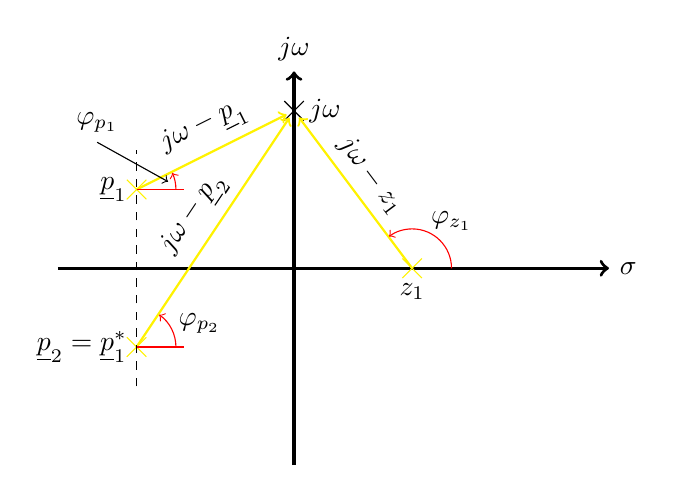
\begin{tikzpicture}

% Koordinatensystem
\begin{scope}[->, very thick]
  \draw (-3,0) -- (4,0) node[right] {$\sigma$};
  \draw (0,-2.5) -- (0,2.5) node[above] {$j\omega$};
\end{scope}

% Punkte p1, p2, z1, jw
\draw (-2,1) node[cross out, draw=yellow] {} node[left] {$\underline{p}_1$};
\draw (-2,-1) node[cross out, draw=yellow] {} node[left] {$\underline{p}_2 = \underline{p}_1^*$};
\draw (1.5,0) node[cross out, draw=yellow] {} node[below=2] {$z_1$};
\draw (0,2) node[cross out, draw] {} node[right=2] {$j\omega$};

% Linien zu jw
\begin{scope}[yellow, ->, thick, shorten >= 3pt]
  \draw (-2,1) -- (0,2) node[midway,above, sloped, black] {$j\omega -\underline{p}_1$};
  \draw (-2,-1) -- (0,2) node[midway, above, sloped, black] {$j\omega - \underline{p}_2$};;
  \draw (1.5,0) -- (0,2) node[midway,above, sloped, black] {$j\omega - z_1$};;
\end{scope}

% Winkel und Beschriftung
\begin{scope}[draw=red]
  \draw (-2,1) -- +(0.6,0); 
  \draw (-2,-1) -- +(0.6,0);
  \begin{scope}[->]
    \draw (-1.5,1) arc (0:25:0.5);
    \draw (-1.5,-1) arc (0:55:0.5);
    \draw (2,-0) arc (0:126:0.5);
  \end{scope}
\end{scope}

\draw (-1.2, -0.7) node {$\varphi_{p_2}$};
\draw (2, 0.6) node {$\varphi_{z_1}$};
\draw[<-] (-1.6,1.1) -- (-2.5,1.6) node[above] {$\varphi_{p_1}$};

% Linie p1, p2
\draw[dashed, very thin]  (-2,-1.5) -- +(0,3);
\end{tikzpicture}